\chapter{Evaluation}

In this chapter, we evaluate our version of incremental induced subgraph isomorphism algorithms.

\subsection{Implementation details}

All algorithms were written in Python. Although Python is not necessarily the right tool 
for implementing high performance algorithms, the main goal of this work was to verify if
we can make significant improvements compared to running VF2++/DAF from scratch by computing
mappings incrementally. To evaluate the correctness of our work, two already existing induced 
subgraph isomorphism implementations were used: networkx's (Python graph library) isomorphism 
module and boost c++ library's vf2\_subgraph\_iso module\cite{boostvf2}. Both modules implement VF2. We 
tried to compare the performance against the original VF2++ implementation \cite{lemonvf2pp}
however it did not produce the same results as the selected baseline implementations. We also
wanted to compare our results to the original DAF implementation, however no sources for the
project were available at time of writing, only a set of pre-compiled binaries \cite{dafbin}
which we did not want to run in the end.

\subsection{Datasets}

We used multiple datasets in our experiments. The first dataset was the Graph Challange\cite{graphchallenge} dataset
which was published by Massachusetts Institute of Technology (MIT) and Amazon Web Services for
the challange. The dataset consists of several large graphs. 

\begin{itemize}
    \item as: network of autonomous systems.
    \item ca-GrQc: collaboration network of general relativity researchers on arxiv.org.
    \item ca-HepTh: collaboration network of high energz physics researchers on arxiv.org.
    \item iso-m2D-m196.A00
    \item iso-m2D-m196.A01
    \item oregon1: peering infromation of autonomous systems in project Route Views of University of Oregon.
\end{itemize}

The other dataset contains multiple generated graphs, namely

\begin{itemize}
    \item random graphs with 1000 nodes and different number of edges between 1500 and 50000. 
    \item scale-free networks generated by the Barabasi-Albert model\cite{barabasimodel}.
\end{itemize}

\subsection{Measurements}

For each of the graphs, the following operations were made. We ran an initial VF2++ and DAF on the given graph $G$
with query graph defined in figure \ref{fig:expq}. Then we randomly deleted and inserted nodes and edges into $G$,
and we measured how much time does it take to incrementally compute the new mapping set. After the graph modifications
we ran our baseline measurement on the resulting graph $G'$, which was networkx's VF2 implementation and we measured
the time it took for the algorithm to finish. We also verified that the number of ismorphisms found by all algorithms
were the same.

\begin{figure}[h!]
	\centering
	\begin {tikzpicture}[auto, node distance=1cm,thick,main node/.style={circle,draw}]
		\node[main node] (0) {\scriptsize$0$};
		\node[main node] (1) [below left=of 0] {\scriptsize$1$};
		\node[main node] (2) [below right=of 0] {\scriptsize$2$};
		\node[main node] (3) [below=of 1] {\scriptsize$3$};
		\node[main node] (4) [below=of 2] {\scriptsize$4$};
		\draw (0) -- (1);
		\draw (0) -- (2);
		\draw (1) -- (2);
		\draw (2) -- (4);
		\draw (3) -- (4);
		\draw (1) -- (3);
	  \end{tikzpicture}
	\caption{Query graph for our experiments}
	\label{fig:expq}
\end{figure}

The first step of our incremental algorithm is to run VF2++ and DAF from scratch. As expected, both algorithms are generally 
faster than VF2. More importantly, the results verify our proposed algorithm. It is significantly faster to update a graph and
incrementally search changes in the mappings set than running a subgraph ismorphism algorithm from scratch. This applies to all
kinds of graphs, even where all three variants semm to struggle, the incremental version still finishes at least one order of
magnitudes earlier.

\begin{figure}
	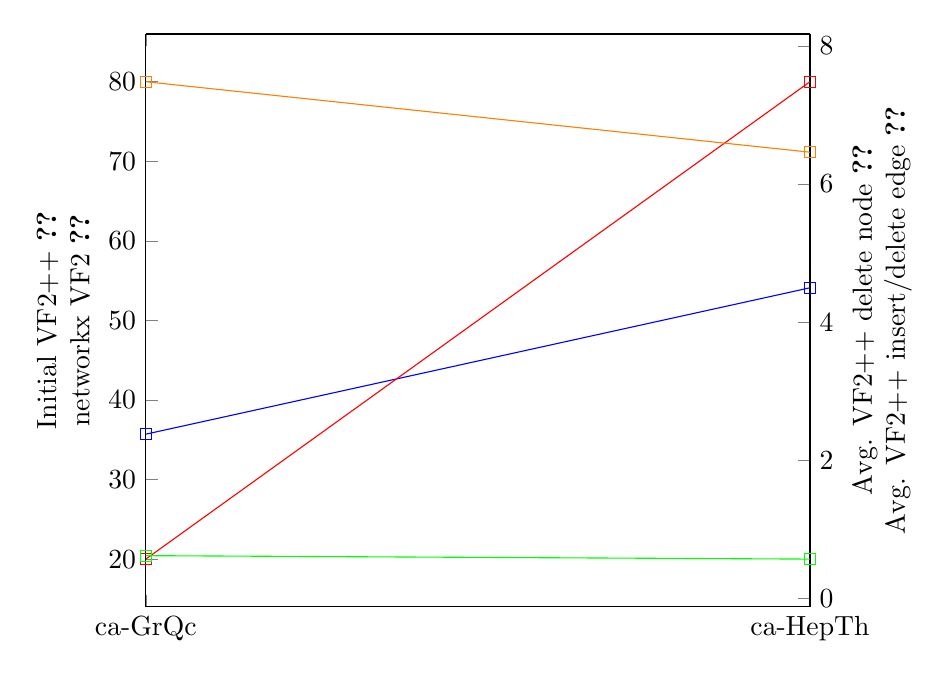
\begin{tikzpicture}
		% let both axes use the same layers
		\pgfplotsset{set layers}
		%
		\begin{axis}[
		scale only axis,
		xmin=0,xmax=1,
		xtick={0,1},
        xticklabels={ca-GrQc,ca-HepTh},
		axis y line*=left,
		ylabel style = {align=center},
		ylabel={Initial VF2++ \ref{plot:vf2ppinitca} \\ networkx VF2 \ref{plot:nxca}},
		]
		\addplot[
            color=blue,
            mark=square,
            ]
            coordinates {
            (0,35.7)(1,54.1)
            };
			\label{plot:vf2ppinitca}
		\addplot[
			color=red,
			mark=square,
			]
			coordinates {
			(0,20)(1,80)
			};
			\label{plot:nxca}
		
		\end{axis}
		%
		\begin{axis}[
		scale only axis,
		xmin=0,xmax=1,
		axis y line*=right,
		axis x line=none,
		ylabel style = {align=center},
		ylabel={Avg. VF2++ delete node \ref{plot:avgnodeca} \\ Avg. VF2++ insert/delete edge \ref{plot:avginsca}},
		]
		\addplot[
			color=green,
            mark=square,
            ]
            coordinates {
            (0,0.62)(1,0.57)
            };
            \label{plot:avgnodeca}
        \addplot[
			color=orange,
            mark=square,
            ]
            coordinates {
            (0,7.48)(1,6.46)
            };
            \label{plot:avginsca}
		\end{axis}
		%
		\end{tikzpicture}
		\caption{Results of ca graphs from Graph Challange}
\end{figure}

\begin{figure}
	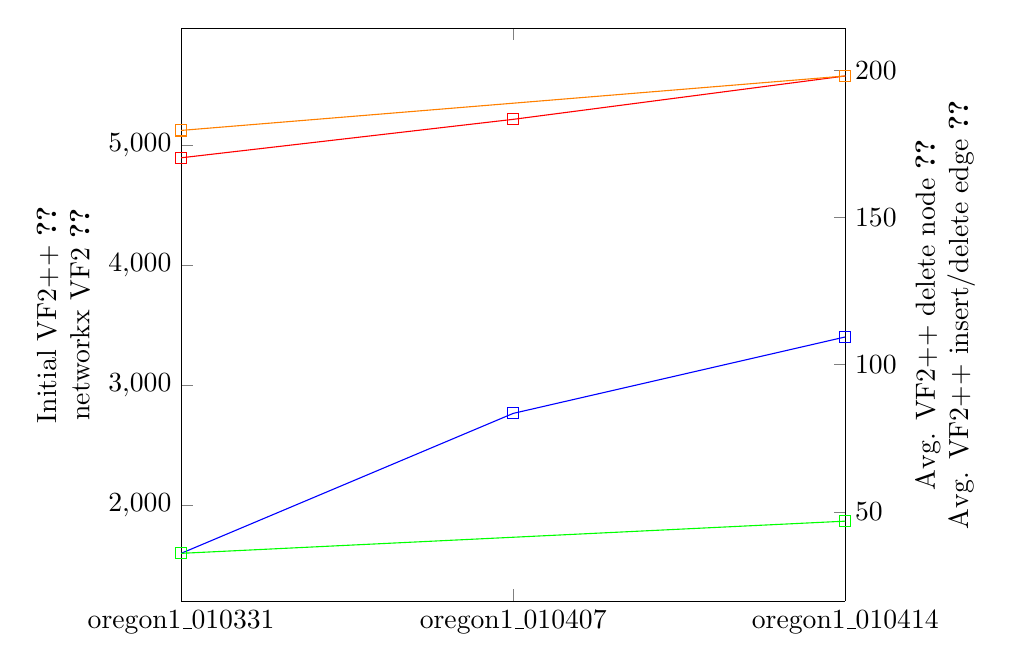
\begin{tikzpicture}
		% let both axes use the same layers
		\pgfplotsset{set layers}
		%
		\begin{axis}[
		scale only axis,
		xmin=0,xmax=2,
		xtick={0,1,2},
        xticklabels={oregon1\_010331,oregon1\_010407, oregon1\_010414},
		axis y line*=left,
		ylabel style = {align=center},
		ylabel={Initial VF2++ \ref{plot:vf2ppinitoregon} \\ networkx VF2 \ref{plot:nxoregon}},
		]
		\addplot[
            color=blue,
            mark=square,
            ]
            coordinates {
            (0,1595)(1,2763)(2,3401)
            };
			\label{plot:vf2ppinitoregon}
		\addplot[
			color=red,
			mark=square,
			]
			coordinates {
			(0,4896)(1,5217)(2,5579)
			};
			\label{plot:nxoregon}		
		\end{axis}
		%
		\begin{axis}[
		scale only axis,
		xmin=0,xmax=1,
		axis y line*=right,
		axis x line=none,
		ylabel style = {align=center},
		ylabel={Avg. VF2++ delete node \ref{plot:avgnodeoregon} \\ Avg. VF2++ insert/delete edge \ref{plot:avginsoregon}},
		]
		\addplot[
			color=green,
            mark=square,
            ]
            coordinates {
            (0,35.94)(1,46.87)(2,58.77)
            };
            \label{plot:avgnodeoregon}
        \addplot[
			color=orange,
            mark=square,
            ]
            coordinates {
            (0,179.54)(1,198.03)(2,236.77)
            };
            \label{plot:avginsoregon}
		\end{axis}
		%
		\end{tikzpicture}
		\caption{Results of oregon graphs from Graph Challange}
\end{figure}

\begin{figure}
	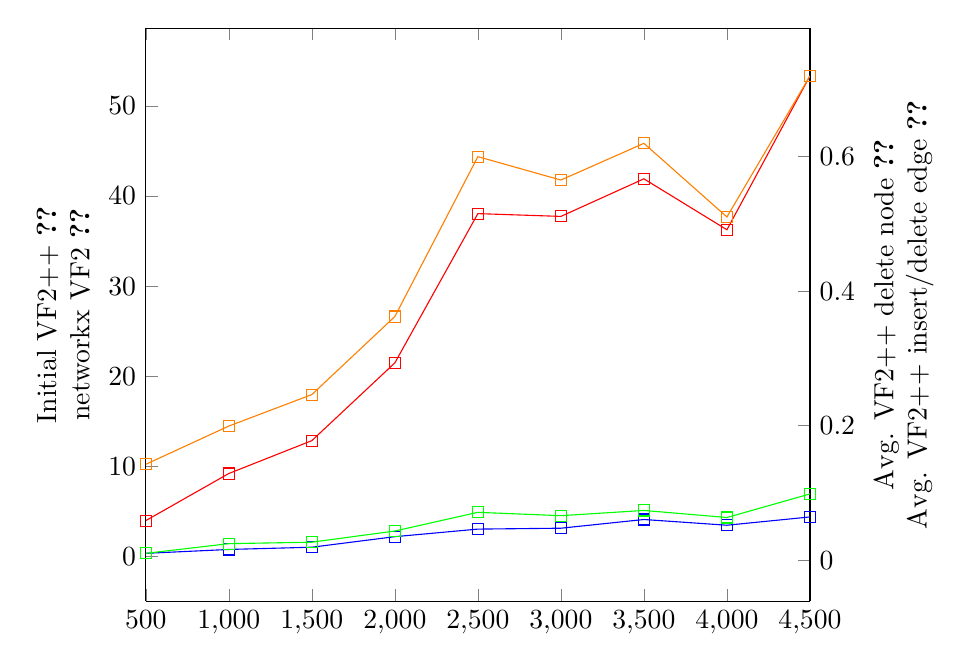
\begin{tikzpicture}
		% let both axes use the same layers
		\pgfplotsset{set layers}
		%
		\begin{axis}[
		scale only axis,
		xmin=500,xmax=4500,
		xtick={500,1000,...,4500},
		axis y line*=left,
		ylabel style = {align=center},
		ylabel={Initial VF2++ \ref{plot:vf2ppinitbar} \\ networkx VF2 \ref{plot:nxbar}},
		]
		\addplot[
            color=blue,
            mark=square,
            ]
            coordinates {
            (500,0.34)(1000,0.77)(1500,1.02)(2000,2.19)(2500,3.03)(3000,3.13)(3500,4.096)(4000,3.46)(4500,4.38)
            };
			\label{plot:vf2ppinitbar}
		\addplot[
			color=red,
			mark=square,
			]
			coordinates {
			(500,3.97)(1000,9.2)(1500,12.85)(2000,21.48)(2500,38.05)(3000,37.74)(3500,41.91)(4000,36.26)(4500,53.33)
			};
			\label{plot:nxbar}		
		\end{axis}
		%
		\begin{axis}[
		scale only axis,
		xmin=500,xmax=4500,
		axis y line*=right,
		axis x line=none,
		ylabel style = {align=center},
		ylabel={Avg. VF2++ delete node \ref{plot:avgnodebar} \\ Avg. VF2++ insert/delete edge \ref{plot:avginsbar}},
		]
		\addplot[
			color=green,
            mark=square,
            ]
            coordinates {
            (500,0.0101)(1000,0.0245)(1500,0.02669)(2000,0.0433)(2500,0.0711)(3000,0.0661)(3500,0.0739)(4000,0.0634)(4500,0.0984)
            };
            \label{plot:avgnodebar}
		\addplot[
			color=orange,
			mark=square,
			]
			coordinates {
			(500,0.1425)(1000,0.1994)(1500,0.2462)(2000,0.3623)(2500,0.6001)(3000,0.5653)(3500,0.6199)(4000,0.5104)(4500,0.7201)
			};
			\label{plot:avginsbar}    
		\end{axis}
		%
		\end{tikzpicture}
		\caption{Results of scale-free graphs generated by Barabasi-model}
\end{figure}